% Optional figure blocks for a report compiled from praesentation/.
% Requires graphicx. Adjust image paths if the main document lives elsewhere.
% This file is not automatically included in any existing report.

\begin{figure}[tb]
  \centering
  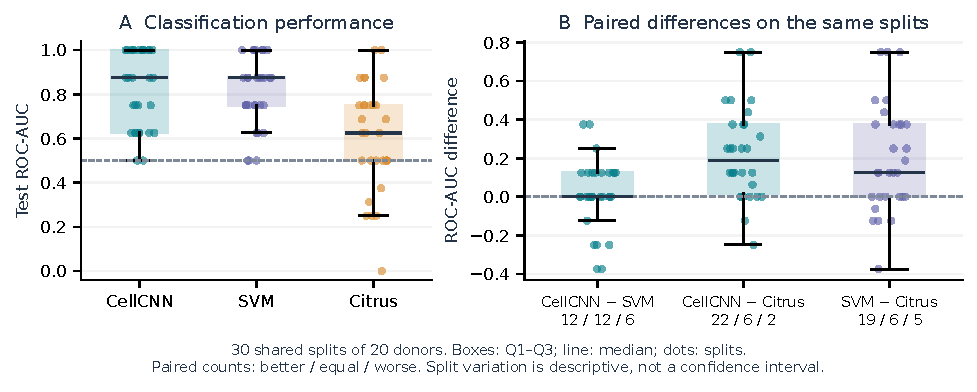
\includegraphics[width=\linewidth]{report_assets/aufgaben_04_05/figures/task4_performance_paired.pdf}
  \caption{Donor-level classification across 30 shared splits of the same
  20 donors, with six test donors per split. Left: test ROC-AUC; right:
  differences between methods evaluated on the same split. Boxes indicate
  the interquartile range, horizontal lines the median, and dots individual
  splits. Counts below paired comparisons denote better/equal/worse splits
  for the first method. Repeated splits describe sensitivity to donor
  partitioning; they are not independent cohorts or confidence intervals.}
  \label{fig:task4-paired-report}
\end{figure}

\begin{figure}[tb]
  \centering
  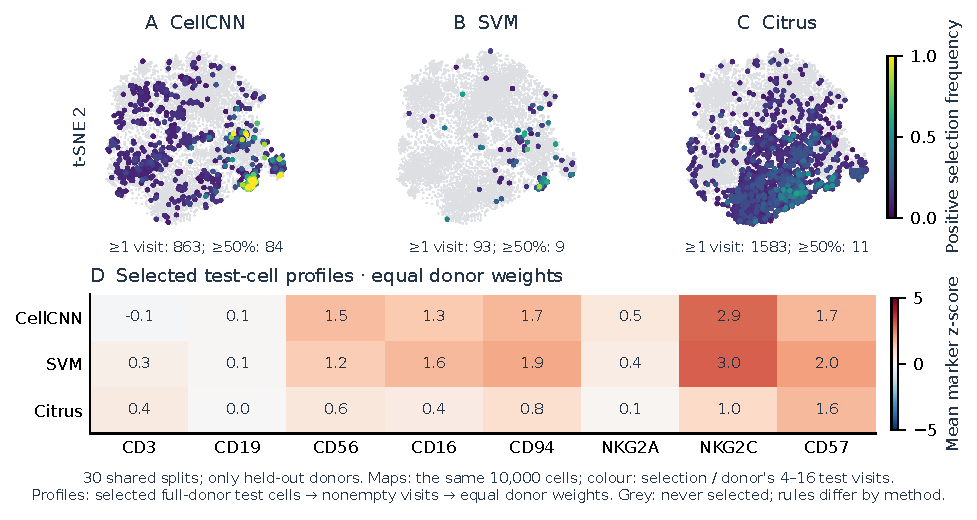
\includegraphics[width=\linewidth]{report_assets/aufgaben_04_05/figures/task5_report_combined.pdf}
  \caption{Cell subsets selected in the CMV-positive direction across 30 shared splits.
  A--C: selection frequency over each donor's 4--16 outer test appearances,
  shown on the same \texttt{gated\_alive} t-SNE reference (10,000 cells,
  500 per donor, perplexity 30). Labels count cells selected at least once
  or in at least half of their test appearances. Grey cells were never
  selected. D: marker profiles of selected full-donor test cells, averaged
  over nonempty visits within donors and then equally across contributing
  donors, on a shared reference z-scale. All three methods use test donors
  only; their selection rules remain method-specific.}
  \label{fig:task5-subsets-report}
\end{figure}
